\documentclass[tikz]{standalone}

\usepackage[sfdefault,light]{roboto}
\usetikzlibrary{shapes, arrows, positioning, backgrounds}
\tikzset{every picture/.style={/utils/exec={\sffamily}}}
\begin{document}
    \begin{tikzpicture} [
                scale=10,
                every node/.style={align=center, draw=none, fill=none, minimum width=2cm},
                legend/.style={font=\small},
            ]
        \node (utilisateur) {
\includegraphics[width=2cm]{images/pc.png}};
        
        \node (internet) [
            below right=.5cm and 1.5cm of utilisateur.east, 
            minimum width=3cm, cloud, draw, fill=white, fill opacity=.6, text opacity=1
        ] {Internet};
        
        \node (serveur1) [above right=.5cm and 1.5cm of internet.east] {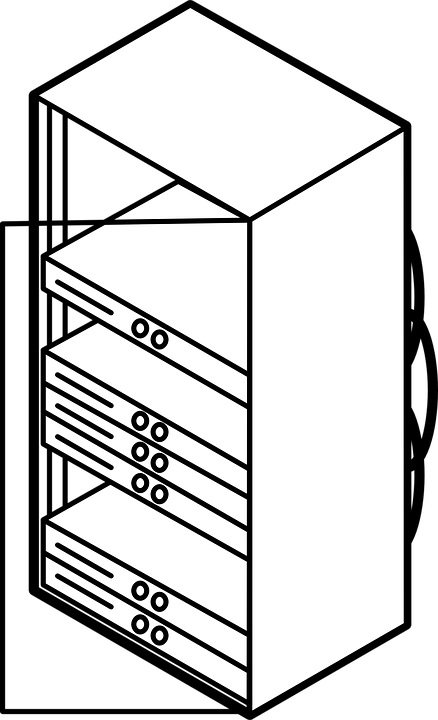
\includegraphics[width=10mm]{images/server.png}};
        \node (serveur2) [below right=.3cm and 3.2cm of internet.east] {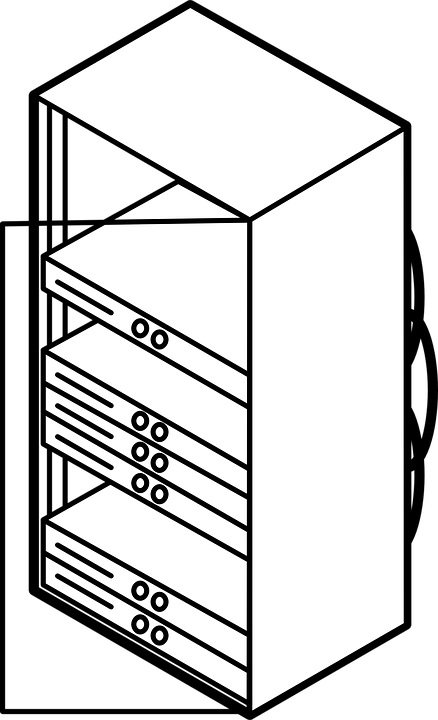
\includegraphics[width=10mm]{images/server.png}};
        \node (serveur3) [below right=1.8cm and .2cm of internet.east] {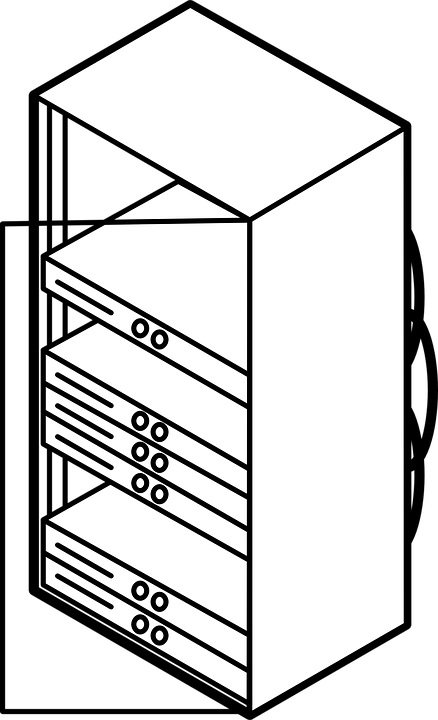
\includegraphics[width=10mm]{images/server.png}};
        
        \node (logo) [below=.1cm of utilisateur] {
            
\includegraphics[width=.5cm]{images/logo_firefox.png} 
            
\includegraphics[width=.5cm]{images/logo_thunderbird.png} 
            
\includegraphics[width=.5cm]{images/logo_whatsapp.png}
        };
        
        \node (utilisateurlegend) [legend, below=.1cm of logo] {utilisateur}; 
        \node (serveur1legend) [legend, below=.1cm of serveur1] {serveur web}; 
        \node (serveur2legend) [legend, below=.1cm of serveur2] {serveur de messagerie \\ électronique}; 
        \node (serveur3legend) [legend, below=.1cm of serveur3] {serveur de messagerie \\ instantanée}; 
        
        \begin{scope}[on background layer]
            \path[<->, ultra thick] (utilisateur) edge [looseness=1, out=330, in=190] (serveur1);
            \path[<->] (utilisateur) edge [looseness=1, out=330, in=160] (serveur2);
            \path[<->] (utilisateur) edge [looseness=1, out=330, in=110] (serveur3);
        \end{scope}
        
        \node (logohtml) [left=of serveur1, xshift=1.5cm, yshift=.5cm] {
\includegraphics[width=.8cm]{images/logo_page_html.png}};
        \node (logomail) [left=of serveur2, xshift=1.5cm, yshift=-.2cm] {
\includegraphics[width=.7cm]{images/logo_mail.png}};
        \node (logomail) [left=of serveur3, xshift=1.8cm, yshift=.8cm] {
\includegraphics[width=.8cm]{images/logo_tchat.png}};
    \end{tikzpicture}
\end{document}